%SICP 1.14习题
\documentclass{article}
\usepackage{CJK}
\usepackage{tikz}
\usepackage{tikz-qtree}
\begin{document}
\begin{CJK}{UTF8}{gkai}
问:画出一棵树,可以用来说明(count-change 11)的函数调用过程。时间和空间增长的阶的增长情况是怎么样的?

答:首先,可用的面额有(1 5 10 25 50)。调用过程可以用(剩余金额, 选择面额)来表示。 当“剩余面额”为0
的时候,就表示程序调用成功。具体的调用过程如下图:

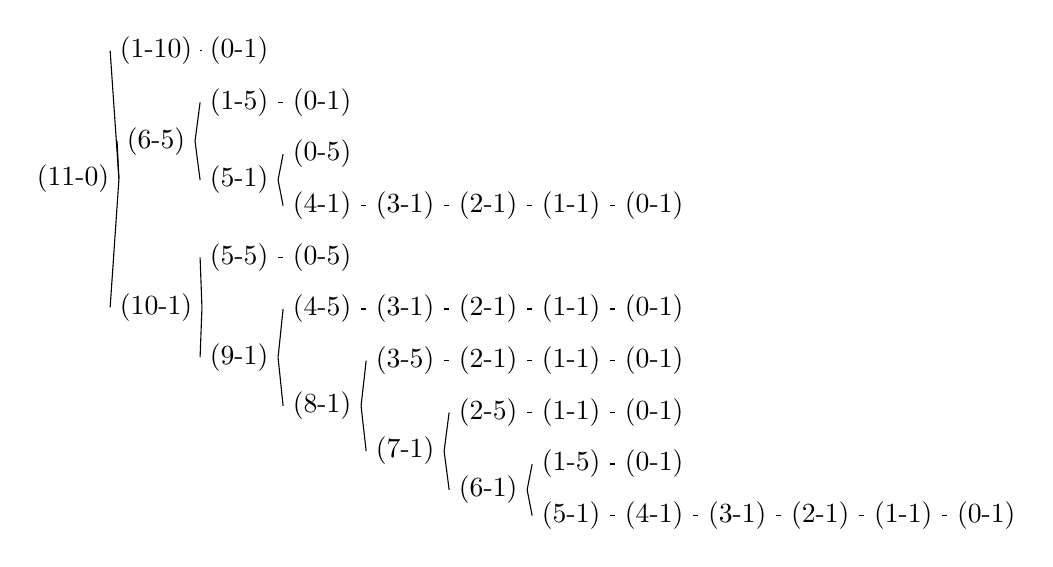
\begin{tikzpicture}[grow=right]
\tikzset {level distance=30pt }
\Tree [ .(11-0) 
               [ .(10-1)
                         [ .(9-1) 
                                  [ .(8-1) 
                                          [ .(7-1) 
                                                   [ .(6-1)
                                                           [ .(5-1)
                                                                    [ .(4-1) [ .(3-1) [ .(2-1) [ .(1-1) (0-1) ]]]]]
                                                           [ .(1-5) (0-1) ]]
                                                   [ .(2-5) [ .(1-1) (0-1) ]]]
                                           [ .(3-5) [ .(2-1) [ .(1-1) (0-1) ]]]]
                                  [ .(4-5) [ .(3-1) [ .(2-1) [ .(1-1) (0-1) ]]]]]  
                         [ .(5-5) (0-5) ]] 
                [ .(6-5) 
                         [ .(5-1) [ .(4-1) [ .(3-1) [ .(2-1) [ .(1-1) (0-1) ]]]] 
                                     (0-5) ] 
                         [ .(1-5) (0-1) ]] 
                [ .(1-10) (0-1) ]]
\end{tikzpicture}

具体的来说,调用的空间占用情况为10, 时间占用情况为40
\end{CJK}
\end{document}